The site offers two ways to find a passage, and they are built to different
units. BM25 \citep{robertson2009} indexes the OCR and returns a page with a
match count. The Jasper index returns an individual text block inside a page.
A page is the finest thing both can name, and it is also what a reader follows
when they click a result, so the comparison is made at page level over
\RetrievalQueries{} queries drawn from the period's own vocabulary, asking the
running services for the top \RetrievalK{} of each.

The two agree far less than one would guess. Mean Jaccard overlap is
\MeanJaccard{} and the median \MedianJaccard{}: of twenty pages returned, three
or so are common to both lists. The most agreed query is
`\MostAgreedQuery{}' at \MostAgreedJ{}, and `\MostDivergentQuery{}' produces
no overlap at all. Figure~\ref{fig:retrieval} shows the full ranking.

\begin{figure}[t]
  \centering
  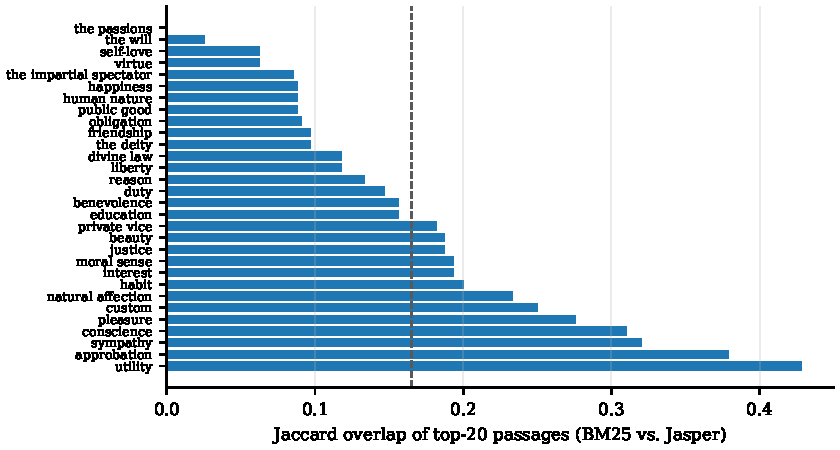
\includegraphics[width=0.94\linewidth]{retrieval_divergence.pdf}
  \caption{Overlap between BM25 and semantic retrieval for the same query, at
           page level, top \RetrievalK{}. The dashed line is the mean. Terms
           whose eighteenth-century use is close to their modern use agree
           most; terms that were technical vocabulary then agree least.}
  \label{fig:retrieval}
\end{figure}

The pattern in that ranking is not random. The queries where the two methods
agree best are the ones whose sense has changed least --- \emph{approbation},
\emph{pleasure}, \emph{custom}. The ones where they diverge most are either
very common words that BM25 matches everywhere while the vectors chase a
particular sense (\emph{the passions}, \emph{the will}, \emph{reason}), or
phrases whose period meaning is carried by surrounding argument rather than
the phrase itself.

A second difference is easier to miss and matters more for a reader. Across
the same queries, BM25 draws its top \RetrievalK{} from \BooksLexMean{}
distinct books on average; the semantic index draws from \BooksSemMean{} ---
roughly half as many. The vector index concentrates. It finds the books that
discuss a topic at length and returns several passages from each, where the
lexical index spreads thinly across everything that happens to use the word.
Neither behaviour is wrong, but a scholar who uses only the semantic index
will systematically see a narrower slice of the library, and will not be told
so. The system's hybrid default, which blends both, exists for this reason;
this measurement is the first quantification of what it is blending.
